\documentclass[Main]{subfiles}

\begin{document}
%-_-_-_-_-_-_-_-_-_-_-_-_-_-_-_-_-_-_-_-_-_-_-_-_-_-_-_-_-_-_-_-_-_-_-_-_-_-_-_-_-_-_-_-_-_-_-_-_-_-_-_-_-_-_-_-_-_-_-_
%-_-_-_-_-_-_-_-_-_-_-_-_-_-_-_-_-_-_-_-_-_-_-_-_-_-_-_-_-_-_-_-_-_-_-_-_-_-_-_-_-_-_-_-_-_-_-_-_-_-_-_-_-_-_-_
%\newpage
\chapter{Lagrangian Systems and Peierls Brackets}
   %introduzione
  In this chapter we will put to good use all the effort invested in the study of mathematical methods for classical field to provide a good notion of Abstract Mechanical system. 
  \emph{Abstract} in the sense that we rely on a refined definition, sufficiently broad to encompass mechanical systems with degrees of freedom both discrete and continuous.
  \\
  Taking advantage of this language will be able to establish the class of systems for which the Peierls' construction procedure  is applicable.
  It will also be possible to contextualize more rigorously each step of the algorithm as shown in the original paper\cite{Peierls1952}.
   
	\section{Abstract Mechanical Systems}
	It's possible to state a mathematical definition sufficiently broad to include all the systems in ordinary analytical mechanics regardless of the cardinality of degrees of freedom  in a unified way.
	
	\begin{definition}[Abstract Evolutive System]
		Pair $(E,P )$ composed of:
		\begin{itemize}
			\item $E \xrightarrow{\pi} M$ \\smooth fiber bundle of typical fiber $Q$ on  manifold $M$ called \emph{"configuration bundle"}.
			\item	$ P : \Gamma^\infty(E) \rightarrow \Gamma^\infty(E)$ \\  operator called \emph{"motion operator"}
		\end{itemize}
	\end{definition}
	This formultation is still very distant from the physical interpretation but has the benift to highlight the minimal mathematical objects which must be fixed in order to specify a mechanical systems.
	
	
	\paragraph{Kinematics}
	%Fibrato Configurazione incompassa la cinematica
	The configuration bundle encompass all the kinematical structure of the system, the pivotal role is played by the smooth sections  which are to be understood as all the possible conformation of the system.

	\begin{notationfix}
		\begin{displaymath}
			\Conf \coloneqq \Gamma^\infty(M,E)
		\end{displaymath}
		Space of kinematic configurations.
	\end{notationfix}

	A section is not a statical configuration, equivalent to a specific point in the configuration space of ordinary classical systems, but has to be seen as a specific realization of the kinematics in the sense of  a complete description of a possible motion.
	At this level of abstraction, since no space-time structure has been specified, terms like stasis and motion must be taken with care .The natural physical interpretation should be clearly manifested through the concrete realization of systems with discrete and continuous degree of freedom.
	
	\begin{observation}[Mathematical structure]
	Mathematically speaking this set should be regarded as an infinite dimensional Manifold. 
	\\
	This framework provides a geometric characterization of the notion of variations as tangent vectors on the the space of kinematic configurations .\cite{Forger2005}
	\end{observation}
	
	\begin{observation}[Coordinate Representation]
	The choice of a chart atlas $\Atlas(M)$ on the base space $M$ and $\Atlas(E)$ on the total space $E$ provides a correspondence between each configuration $\gamma \in \Conf$ and family of smooth real functions $\{f_{\alpha \beta}:A_\alpha \subset \Real^m \rightarrow \Real^q \}$.
	The process is trivial:
	\begin{displaymath}
		\gamma \in \Conf \mapsto \{f_{A,U}=\psi_U \circ \gamma \circ \psi_A^{-1} \vert (A,\psi_A) \in \Atlas(M), (U,\psi_U)\in \Atlas(E)   \}
	\end{displaymath}
	
	%	$\forall (A,\psi_A)$ local chart on $M$ and $(U,\psi_U)$ local chart on $E$ such that $\gamma(A) \cap U \neq \emptyset$ $f_{A,U}=\psi_U \circ \gamma \circ \psi_A^{-1}$

	Since the whole section as a global object is quite difficult to handle is customary in field theory to work in the more practical local representation. 
	\end{observation}	
	
	\begin{observation}[Further specification of the system's kinematics]
	 	The general formalism doesn't require any other structure to be carried forward.
	 	Additional structure on the fiber , the base or the whole bundle are to be prescribed in order to specify a precise physical model, e.g. the spin structure on $E$ for the Dirac Field.\cite{Benini}
	 \end{observation}	
	
	\paragraph{Dynamics}
	The operator $P$ is the object that contains all the information about the dynamic evolution of the system.
	It has the role to select the dinamically compatible configuration among all the admissible kinematic configurations of $\Conf$, exactly as it happens in analytical mechanics where the dynamic equations shape the natural motions.
	\begin{notationfix}
		Provided an equations of motion operator
		\begin{displaymath}
			P: \Conf \rightarrow \Conf
		\end{displaymath}
		The space
		\begin{displaymath}
		\Sol \coloneqq \ker(P) \subset \Conf
		\end{displaymath}
		containing all the smooth solutions is called \emph{"Space of Dynamical Configurations"}.
	\end{notationfix}
	
	\begin{figure}[h!]
		\centering
		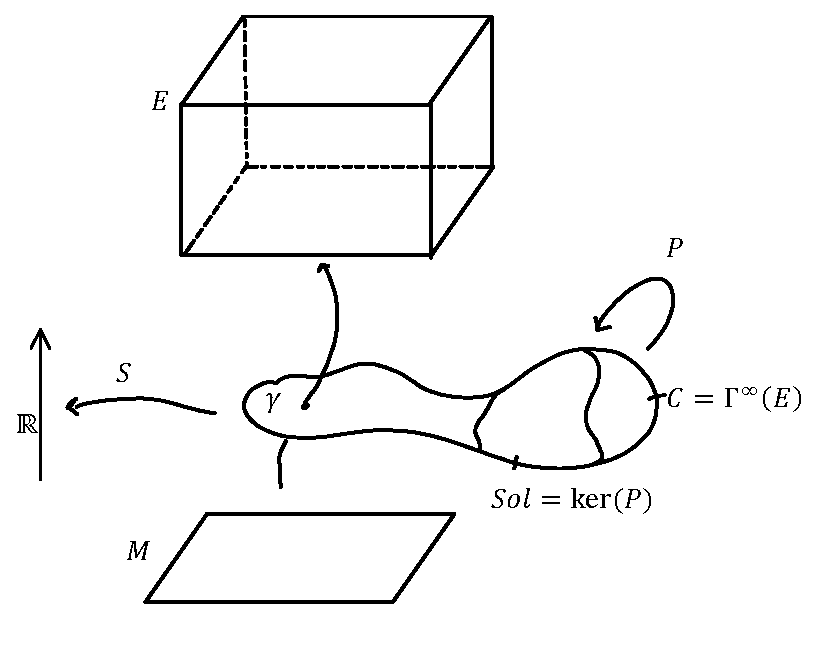
\includegraphics[width=0.5\textwidth]{Pictures/AbstractFieldTheory} 
		 	 	\caption{Mathematimatical framework of the mechanics of abstract systems. }
	\end{figure}	
	
	\subsection{Lagrangian Dynamics}	
	Lagrangian systems constitute a subclass of the abstact mechanical systems of more practical interest:	
		\begin{definition}[Lagrangian System]
	Pair $(E, \mathcal{L} )$ composed of:
		\begin{itemize}
			\item $E \xrightarrow{\pi} M$ \\smooth fiber bundle of typical fiber $Q$ on the oriented manifold $(M,\mathfrak{o})$ called \emph{"configuration bundle"}.
			\item	$ \Lagrangian : J^r E \rightarrow \wedge^m T^*M$ \\bundle-morphism from the r-th Jet Bundle to  the top-dimensionial forms bundle over the base manifold $M$  called \emph{"Lagrangian density"} or simply \emph{"Lagrangian"} of r-th order.
		\end{itemize}
	\end{definition}	
	
	\begin{NB}
		IIn what follows all the systems considered will be exclusively of first order.
	\end{NB}	
	
	
	%la lagrangiana incompassa la dinamica
	In this case is the Lagrangian density the object containing all the information about the dynamic evolution of the system.

	%In Layman terms la lagrangiana  è un qualcosa che può essere integrato sopra la varietà
	In order to reconstruct the system's dynamic from the Lagrangian density has to be understood the mathematical nature of $\Lagrangian$.
	$\Lagrangian$ maps point $q_p$ on the fiber $J^r_p E$ to a m-form on $T_p M$.
	Recalling the definition of jet bundles is clear that for each smooth section on $E$ is associated a smooth section on the b$J^rE$ :
	\begin{displaymath}
		\phi \in \Gamma^\infty (E) \mapsto (\phi, \partial_\mu \phi, \partial_{\mu, \nu} \phi , \ldots \partial_{\vec{\alpha}}\phi)
	\end{displaymath}
	where  $\vec{\alpha}$ is a multi-index of length r.
	The correspondence is not univocal since sections equal up to the r-th order define the same jet section.
	The smoothness of $\Lagrangian$ ensure that each jet bundle section is mapped to a smooth section in the top-forms bundle i.e. the most general integrable object on a orientable manifold.
	
	%la classe delle densità lagrangiane
	It should be clear that $\Lagrangian$ is a specific choice among the vast class of functions suitable to be a good Lagrangian density over the  Configuration Bundle $E$:
	\begin{definition}[Lagrangian Density on the bundle $E$]
		\begin{displaymath}
			\Lag^r (E) \coloneqq \hom\biggr(J^r E,\quad \bigwedge^m( T^*M)\biggr)  \cong \big\{f:\Gamma^\infty(J^r E) \rightarrow \Omega^m(M)  \big\}
		\end{displaymath}
	(where $\Omega^m(M)$ is the common name for $\Gamma^\infty \big( \bigwedge^m( T^*M) \big)$ in the context of Grassmann algebras.)
	The equivalence states the fact that a bundle-morphism induce a mapping between the sections.
	\end{definition}
	 this choice fix the "Dynamical identity" of the considered system.
	\begin{proposition}
		$\Lag^r(E)$ has an obvious vector space structure inherited by the linear structure of $\Omega(M)$.
	\end{proposition}
	
	
	Thanks to the correspondence between a section $\phi \in \Conf$ and his r-th jet, it's possible to consider the Lagrangian as directly acting on the kinematic configurations.
	In layman terms the image  $\Lagrangian [ \phi ] \textrm{d}\mu$ , where $\textrm{d}\mu$ is the measure associated to the orientation $\mathfrak{o}$, is something that can be measured over the whole base space. 
	\\
	This property suggests the introduction of the class of associated functionals:
	\begin{definition}[Lagrangian functional]
		Is a functional on $\Conf$ with values on regular distribution over M associated to the generic $\Lagrangian \in \Lag$.	
		\begin{displaymath}
			\mathcal{O}_\Lagrangian : \Conf \rightarrow \big( C^\infty_0(M) \big)'
		\end{displaymath}			
			Such that the lagrangian functional associated to $\Lagrangian$, valued on the configuration $\phi \in \Conf$ and tested on the test-function $f \in C^\infty_0(M)$ it's given by:
		\begin{displaymath}
			\mathcal{O}_\Lagrangian [\phi] (f) = \int_M \Lagrangian [\phi] f \textrm{d}\mu
		\end{displaymath}		
	\end{definition}	
	
	\begin{proposition}
		As a distribution $\mathcal{O}_\Lagrangian [\phi] (f) $ is necessarily linear in the test-functions entry but not in the configurations entry.	
	\end{proposition}	
	
	\begin{observation}
		The choice of the image of $\mathcal{O}_\Lagrangian$ as a distribution it's a necessary precaution to ensure that functional is \emph{"convergent"} whatever is the configuration on which is evaluated.
		In fact, despite $\Lagrangian [ \phi ]$ is integrable with respect to the measure $\textrm{d}\mu$, it's not necessary summable if the support of the configuration $\phi$ becomes arbitrarily large.
		\\
		This is a simple consequence of the well known sequence of inclusions:
		\begin{displaymath}
			\Lagrangian [ \phi ] \in C^\infty_0(M) \subset L^1_{\textrm{loc}}(M,\mu) \supsetneqq  L^1(M,\mu) 
		\end{displaymath}
		of the functional analysis .
		Indeed, the functional
		\begin{displaymath}
			\mathcal{O}_\Lagrangian [\phi]= \int_{\supp(\phi)} \Lagrangian [\phi] \textrm{d}\mu
		\end{displaymath}
		is well defined for all $\Lagrangian \in \Lag^r(E)$ only over the compactly supported sections. 
		To take account of the global sections it's sufficient to dampen the integral multiplying the integrand with an arbitrary test-function.
	%il funzionale lagrangiana totale e azione
	\end{observation}
	
	\begin{notationfix}
		When calculated for the specific density of the Lagrangian system $\mathcal{O}_\Lagrangian$ takes the name of \emph{Action} or \emph{Total Lagrangian}. 
	\end{notationfix}

	The introduction of the Lagrangian density is meaningless without the prescription of a dynamical principle which allows to determine univocally a differential operator $P$ on the kinematics configurations space $\Conf$.
	This fundamental principle is the \emph{least action principle}.
	A proper justification of this claim should require the presentation of the differential calculus on the infinite dimensional manifolds $\Conf$. 
	Jumping straight to the conclusion we can state this correspondence as a principle  in term of a function which assign for all lagrangian densities an operator on the kinematic configurations space. In the case of first order lagrangian we define
	\begin{definition}[Euler-Lagrange operator]
		It's the differential operator
		\begin{displaymath}
			Q_\chi : \Conf \rightarrow \Conf
		\end{displaymath}
		relative to the lagrangian density $\chi \in \Lag^1(E)$, such that:
		\begin{equation}
			Q_\chi (\gamma) = \Biggr( \partial_\mu \biggr( \frac{\partial \chi}{\partial(\partial_\mu \phi)} \biggr\vert_\gamma \biggr) - \frac{\partial \chi}{\partial \phi}\biggr\vert_\gamma \Biggr) \qquad \forall \gamma \in \Conf
		\end{equation}
		(where 	$\biggr( \frac{\partial \chi}{\partial(\partial_\mu \phi)}$ is the be intended as the lagrangian density constructed differentiating $\chi(\phi, \partial_\mu)$ as an ordinary function treating its functional entries as an usual scalar variable.)
	\end{definition}
	
	\begin{observation}
		The whole theory of both Lagrangian densities class and Euler-Lagrange equation could be stated in a more syntetic way in terms of the Grassmann-graded variational bicomplex.\cite{Giachetta2009}\cite{Sardanashvily}
	\end{observation}
	
		

%-_-_-_-_-_-_-_-_-_-_-_-_-_-_-_-_-_-_-_-_-_-_-_-_-_-_-_-_-_-_-_-_-_-_-_-_-_-_-_-_-_-_-_-_-_-_-_-_-_-_-_-_-_-_-_-_-_-_-_
%-_-_-_-_-_-_-_-_-_-_-_-_-_-_-_-_-_-_-_-_-_-_-_-_-_-_-_-_-_-_-_-_-_-_-_-_-_-_-_-_-_-_-_-_-_-_-_-_-_-_-_-_-_-_-_
%\newpage
	\section{Concrete Realization}
	In the previous section we claim that the abstract definition of Lagrangian systems is broad enough to encompass all the classical lagrangian systems with both discrete degrees of freedom, like particles, and continuous degree of freedom, like fluids or fields.
	Let' show two of the most significant examples.
	%esibiamo quanto è ampia la nostra definizione
	
	
	
		\subsection{Classical Field Theory}
		Basically a \emph{Fields System} is nothing more than an abstract Field System $(E,P)$ where the base space $M$  is a suitable Spacetime manifold\cite{Bar}. At this stage the question about the Lagrangian nature of the dynamics is purely ancillary.
		\\		
		The idea of taking bundles on a space-time manifold is physically intuitive, kinematically speaking a fields configuration is simply the association of some element of the fiber $Q $ for each point of the space-time $M$.
		
		However, there are two more requirements that are often prescribed in commonly studied field theories.
		\paragraph{Linear Sistem Condition}		
			\begin{itemize}
				 \item The configuration bundle $E\xrightarrow{\pi} M$ is a \underline{vector bundle}.
			\end{itemize}
			Even if it might make sense to speak of nonlinear fields in some more general context, this condition it's a necessary element in case some form of the \emph{superposition principles} as to be taken in account.
			Obviously this hypothesis is not sufficient to formulate the principle in the strong classical way, i.e.:"the response at a given place and time caused by two or more stimuli is the sum of the responses which would have been caused by each stimulus individually" mostly because only free systems can be considered at this stage and any statement about stimulus can make sense.
			\\
			However It assure that $\Conf$ is a vector space and , in conjunction with the linearity of motion operator $P$, $\Sol= \ker(P)$ is a linear subspace.		
			In other words every linear combination of kinematic configuration it's still a kinematic configuration.
			 
		\paragraph{Propagative Dynamic Condition}
		\begin{itemize}
			 \item The base manifold $M$ is a \underline{Globally Hyperbolic Spacetime}.
			 \item The motion operator $P$ is \underline{PDE-hyperbolic}.
		\end{itemize}
		The first condition ensures the existence of Cauchy surfaces and therefore permits to state  \emph{Cauchy Problems} assigning an initial data on such regions.
		Furthermore, PDE-hyperbolicity of the motion operator $P$ guarantees that for every Cauchy surface $\Sigma \subset M$ the corresponding initial data problem is well posed, that is:
			\begin{equation}\label{CauchyProblem}
				\begin{cases} P u = 0 \\ u = u_0 \\ \nabla_{\vec{n}}u= u_1 \end{cases}
			\end{equation}
			admit a unique solution $u\in \Gamma(E)$ for all $(u_0, u_1) \in \Gamma (\Sigma )\times \Gamma (\Sigma )$.
			\\
			This suggests the following definition:
			\begin{notationfix}
				The set of all the smooth initial data which can be given on the Cauchy Surface $\Sigma$ is:
				$\Data(\Sigma)  \coloneqq \biggr \{ (f_0,f_1) \big \vert f_i \in \Gamma^\infty(\Sigma)\biggr\}  \equiv  \Gamma^\infty(\Sigma) \times \Gamma^\infty(\Sigma)$
			\end{notationfix}
			\begin{observation}
				$\Data(\Sigma)$ inherit the linear structure of its component $ \Gamma^\infty(\Sigma)$.
			\end{observation}	
			In this term the well-posedness of the Cauchy problem can be stated as follow:

			\begin{proposition}
				The map $ 	 \SolMap : \Data (\Sigma ) \rightarrow \Sol $ which assign to $(u_0, u_1)\in \Data(\Sigma)$ the unique solution of the cauchy problem \ref{CauchyProblem} is linear and bijective.
			\end{proposition}
			
			Since any solution, when restricted to a generic Cauchy surface $\Sigma'$, determines another pair of initial data, i.e.:
			\begin{displaymath}
				\phi \equiv \SolMap (\phi \vert_{\Sigma'}, \nabla_{\vec{n'}}\phi	 \vert_{\Sigma'} )	\quad \forall \phi\in \Sol
			\end{displaymath}						
			we can define the set of initial data regardless of the particular Cauchy surface:			
			
			\begin{definition}[Set of smooth initial Data]
				\begin{displaymath}
					\Data  \coloneqq \frac{\bigsqcup\limits_{\Sigma \in \PowerSet_C(M)}\Data(\Sigma)}{\sim} 
				\end{displaymath}
				where $\sim$ is such that:
				\begin{displaymath}
					(f_0, f_1)|_\Sigma \sim (g_0, g_1)|_{\Sigma'} \; \Leftrightarrow \; \SolMap(f_0,f_1) =  \SolMap(g_0,g_1) 
				\end{displaymath}
				\footnotesize{ Initial data, associated with different surface, are similar if they lead to the same solution.}	
			\end{definition}
			
			\begin{proposition}
				$\Data$ is still a vector space.
			\end{proposition}
			\begin{proof}
				It's sufficient to prove that:
				\begin{displaymath}
					\big[ \phi_a + \phi_b \big] = \big[ \phi_a \big] + \big[ \phi_b \big]
				\end{displaymath}
				where $[\phi]= \big\{(\phi\vert_\Sigma , \nabla_{\vec{n}}\phi \vert_\Sigma) \big\vert \Sigma \in \PowerSet_C \big\}$.
				In fact:
				\begin{align*}
					 \SolMap_{\Sigma'}\big([(a',b')] + [(c',d')] \big)=\SolMap_\Sigma\big([(a,b)] + [(c,d)] \big) = \SolMap_\Sigma\big([(a,b)] \big)+ \SolMap_\Sigma\big([(c,d)] \big) =\\
					 =\SolMap_{\Sigma'}\big([(a',b')] \big)+ \SolMap_{\Sigma'}\big([(c',d')] \big) = \SolMap_{\Sigma'}\big([(a',b')] +[(c',d')] \big)
				\end{align*}

			\end{proof}
			\begin{corollary}
				The function  $ 	 \mathbb{s} : \Data (\Sigma ) \rightarrow \Sol $ which map every equivalence class to the associated solution is linear and bijective.
			\end{corollary}
		\begin{observation}
			The Propagative dynamic condition  is the main ingredient in the \emph{initial data quantization} procedure\cite{Wald1994}.	
		\end{observation}	
	
	
		\paragraph{Green-Hyperbolic Dynamic Condition}
		\begin{itemize}
			\item The dynamic is generated by a \underline{Lagrangian}, i.e.  $P= Q_\Lagrangian$.
			\item The motion operator $P$ is a \underline{Green Hyperbolic} L.P.D.O.
		\end{itemize}
		It's customary in Algebraic quantum field theory to identify quantizable systems through this condition.
		In fact this condition is a necessary hypothesis to carry on the Peierls construction and the brackets underlie to the definition of the classical symplectic structure.
		\\
		We remark that Green-hyperbolic operators are not necessarily hyperbolic in any PDE-sense, therefore the last two condition are not equivalent.
			 
		\begin{example}
		It's straightforward  to frame the well-known \emph{Real Scalar Field on curved background} inside this abstract picture:
			\begin{center}\begin{tabular}{|l|c|}
			\hline
			Configuration bundle & real scalar field: $F \equiv \Real$\\
													& curved background: $M$ is globally hyperbolic\\
			\hline
			Kinematic Configurations & $\Conf = C^\infty(M,\Real)$\\
			\hline
			Motion Operator			&  $P=\square_M + m^2 + \xi R$ \\
													& normally hyperbolic operator\\
			\hline
			\end{tabular}\end{center}
			Where $P$ is the Klein-Gordon Operator: $\xi$ and $m^2$ are two real numbers, $R$ stands for the scalar curvature build out of $g$ and $\square_M \coloneqq g^ab \nabla_a \nabla_b$ is the d'Alambert operator associated to the Levi-Civita connection.	
			
		Note that this system satisfies all the above three condition.
		\end{example}
	



		\subsection{Finite Degree systems as a Field}\label{MechanicsAsAField}
			With a little more effort is possible to see every ordinary mechanic system  -with discrete degrees of freedom- as a special case of classical field.
			
			Consider a lagrangian system $(Q, L)$ with configuration space $Q$ and Lagrangian function $L: TQ\rightarrow \Real$.
			
			Remembering the intuitive meaning of $Q$ as set of all the statical conformation of the system, it's natural to read as kinematic configuration all and only the trajectories compatible with the constraints.
			In other words the space of kinematic configurations is the set of all the parametrized smooth curves on $Q$:
			\begin{displaymath}
				\Conf = C^\infty(\Real,Q)
			\end{displaymath}
			Therefore, the configuration bundle of this system is the trivial smooth bundle:
			\begin{displaymath}
				E= ( \Real\times Q, \pi, \Real)
			\end{displaymath}
			of typical fiber $Q$, since the corresponding space of sections coincides to  the required configuration space:
			\begin{displaymath}
				\Gamma^\infty(E) \equiv C^\infty(\Real,Q)
			\end{displaymath}

			Also the "field theoretic" picture of the dynamic is not difficult to achieve.
			It's enough to recall how the Euler-Lagrange of ordinary mechanical system can be derived from the \emph{least action principle}:
			\begin{quotation}
				\textbf{Least Action Principle:}
				The natural motions of the mechanical system $(Q,L)$ are the stationary points of the action functional:
				\begin{displaymath}
					S [\gamma]= \int_\Real L(t,\gamma^i, \dot{\gamma}^i) dt
				\end{displaymath}
				constructed from the Lagrangian of the system.
			\end{quotation}
			Remembering that we have interpreted the space $\Real$ of the parameter $t$ as the base manifold of the configuration bundle $E$, it's immediate to see $S$ as the \emph{Total Lagrangian} related to the lagrangian density:
			\begin{displaymath}
				\Lagrangian[\gamma] \coloneqq L \circ \big( \gamma \big)^{\big\uparrow} dt
			\end{displaymath}
			obtained evaluating the ordinary Lagrangian on the lifted curve $\gamma^\uparrow$ (lift of $\gamma\in \Conf$ from $Q$ to $TQ$).
		


		Summing up, the mathematical structure of such mechanical system is enconded as follows:
			
			\begin{center}\begin{tabular}{|l|c|}
			\hline
			Configuration bundle & Trivial bundle  $E= Q \times \Real$\\
													& Base manifold: $M=\Real$\\
			\hline
			Kinematic Configurations &  $\Conf=C^\infty(\Real,Q)$\\
			\hline
			Lagrangian Density		&	$\Lagrangian  [\gamma] \coloneqq \big( L \circ	\gamma^\uparrow \big) dt  = L(t,\gamma^i,\dot{\gamma}^i) dt$\\
			\hline
			Motion Operator			&  $P=Q_\Lagrangian \equiv \frac{d}{dt}\big(\frac{\partial}{\partial \dot{x}^i}L\big)-\frac{\partial}{\partial x^i}L $\\
													& normally hyperbolic operator (\danger ?)\\
			\hline
			\end{tabular}\end{center}
			
			Considering that the space $M$ is trivially globally hyperbolic, since every point $t\in\Real$ is a genuine "Cauchy Surface", it's evident how this system can be seen as a special case of field theory: a "field of curves".
			\begin{observation}
				Unless the configuration space is a vector space, the corresponding field theory cannot be linear.
			\end{observation}		
		
%-_-_-_-_-_-_-_-_-_-_-_-_-_-_-_-_-_-_-_-_-_-_-_-_-_-_-_-_-_-_-_-_-_-_-_-_-_-_-_-_-_-_-_-_-_-_-_-_-_-_-_-_-_-_-_
%\newpage
	\section{Hamiltonian of Finite Degree systems}
		The picture of the systems with discrete degrees of freedom as a field brings out only a part of the typical mathematical ingredients proper of the \emph{Geometric} approach to the classical mechanics

		\begin{figure}[h!]
		\centering
		\begin{minipage}{0.45\textwidth}
			\centering
			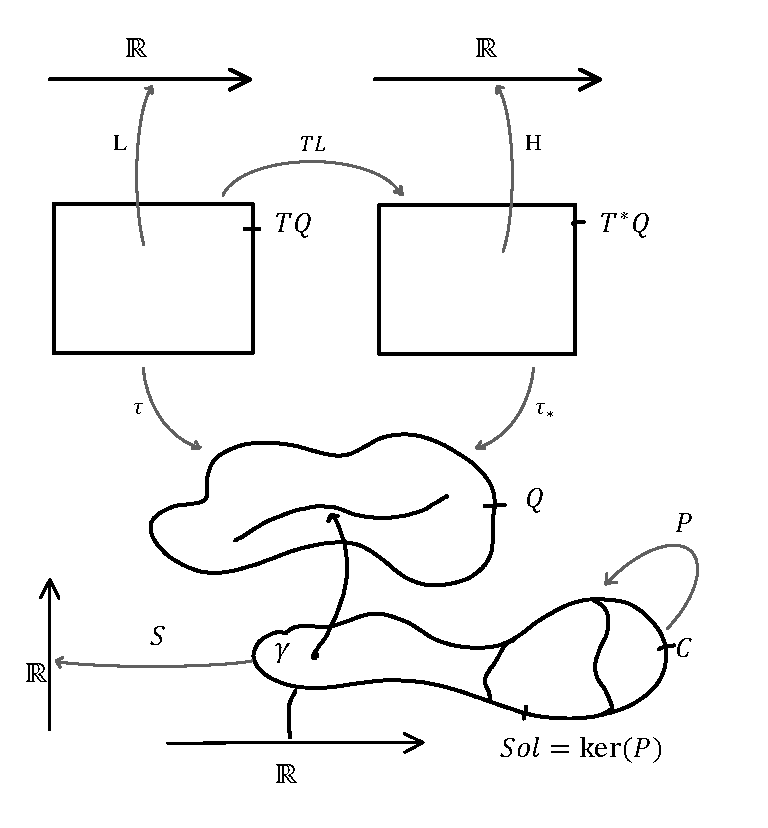
\includegraphics[width=\textwidth]{Pictures/GeoMecFrame} 
			%\caption{first figure}
		\end{minipage}\hfill
		\begin{minipage}{0.45\textwidth}
			\centering
			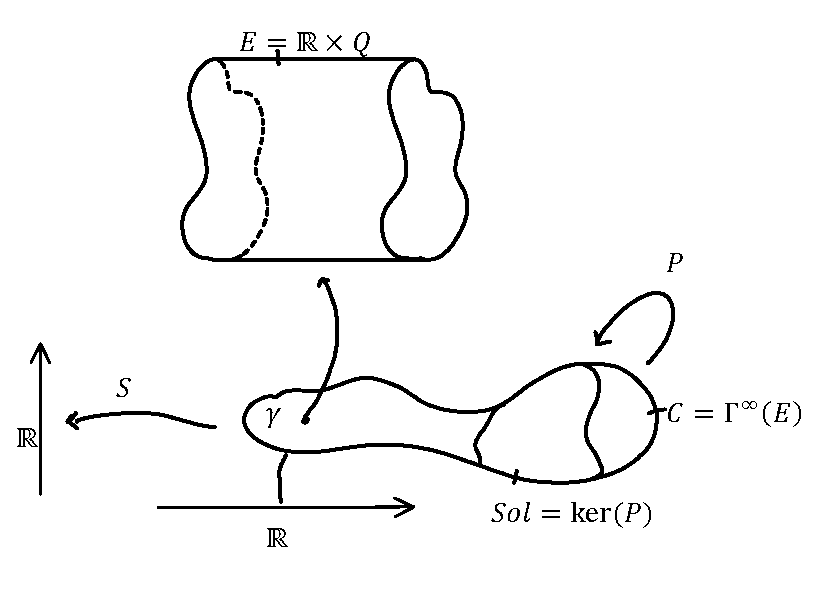
\includegraphics[width=\textwidth]{Pictures/FieMecFrame} 
			%\caption{second figure}
		\end{minipage}
		\caption{An "impressionistic comparison"  between the mathematical framework of geometrical mechanics and  the field-theoretic picture}
		\end{figure}
	
	For example we have totally overlook to mention the hamiltonian formalism in the case of field.
	Even though it should be possible, in the spirit of what has been done for Lagrangian picture, to extend the canonical treatment to include systems with continuous degrees of freedom (see for example \cite{Giachetta1999}).
	We will not expand this topic since the protagonist of this paper is essentially a single-particle system.
	
	However in the next chapter we will need to realize a field-theoretic versions of some Canonical objects.
	Let's briefly review their finite dimensional version.
	
			\paragraph{Phase Space}
		We recalled in chapter 1 the definition of \emph{Phase Space} in ordinary classical mechanics as the cotangent bundle $T^*Q$ of the classical configuration space $Q$.
		We showed that every classical phase space is symplectic trough the natural Poincarè form.
		However, every quantization procedure require a modification of this standard symplectic form in order to implement the canonical commutation rules.
	
	This leads us to the abstract formulation for the Hamiltonian systems\cite{Abraham1978}:
	
	\begin{definition}[Hamiltonian System]
	 $(\mathcal{M},\omega, H)$ 3.3.1 fomm
	\end{definition}
	
	\begin{observation}
		In classical mechanics Hamiltonian systems could be seen as a subset of Lagrangian systems.
		\\
		The key is the definition of the Legendre Map $TL: TQ \rightarrow T^*Q$. 
		Only in the case that the Lagrangian$L$  is \emph{hyperegular}, i.e. $TL$ is a diffeomorphism, is possible to push-forward $L$ to give a proper Hamiltonian on $\Phase=T^*Q$. (see for example \cite{Abraham1978}		
	\end{observation}	
	Remember that there's an important theorem attributed to Darboux that state that, at least locally, every symplectic form can be coordinated as the ...canonical coordinate
	\begin{theorem}[Darboux]
	3.2.2 fomm
	\end{theorem}
	
	\paragraph{Classical Observables}
		Observables in classical mechanics are represented by real valued smooth function on $\Phase$
	\begin{notationfix}
		The \emph{Classical Observables} space is denoted as:
		\begin{displaymath}
			\Obs \equiv		C^\infty(\Phase,\Real)
		\end{displaymath}
	\end{notationfix}
	\begin{observation}
		Trivially, the space  $C^\infty(\Phase,\Real)$ of smooth real valued function on $\Phase$,  inherits the structure of commutive algebra over $\Real$ from its codomain $\Real$.
	\end{observation}
	The symplectic structure on $\Phase$ give rise to an alternative algebraic structure on the vector space of observables.
	At first it is necessary to introduce the Hamiltonian fields:
	\begin{definition}[Hamiltonian field]
	3.3.1 fomm
	\end{definition}
	from that follows the definition of the bracket:
	\begin{definition}[Poisson Bracket]
	3.3.11 fomm
	\end{definition}	
	
	\begin{proposition}[Symplectic char representation]
	3.3.14 fomm
	\end{proposition}

	
	\subsection{Linear dynamical systems}	
		
	Most of the physical systems that are encountered in the theory of fields are linear.
	 da qui si va su Wald
	
	Of course is possible to come across linear systems even in ordinary mechanics. 
	In that case the the difference between the underlying geometric entities tend to fade out as a consequence of the flatness of the configuration space.
	
	\begin{Warning}
	Da riempire: devo dire che 
	\begin{itemize}
		\item Q è piatto
		\item TQ è fibrato vettoriale
		\item Q si identifica con il tangente quindi la forma simplettica è definita direttamente sulle configurazioni
		\item ecc vedere primo capitolo wald
	\end{itemize}
	\end{Warning}


%-_-_-_-_-_-_-_-_-_-_-_-_-_-_-_-_-_-_-_-_-_-_-_-_-_-_-_-_-_-_-_-_-_-_-_-_-_-_-_-_-_-_-_-_-_-_-_-_-_-_-_-_-_-_-_-_-_-_-_
%-_-_-_-_-_-_-_-_-_-_-_-_-_-_-_-_-_-_-_-_-_-_-_-_-_-_-_-_-_-_-_-_-_-_-_-_-_-_-_-_-_-_-_-_-_-_-_-_-_-_-_-_-_-_-_
%\newpage
	\section{Peierls Brackets}
		Purpose of the Peierls' procedure is to provide a bilinear form on the space of Lagrangian densities with time-compact support.
		This form induces a pre-symplectic structure on suitable subspaces of functionals to which can be recognized the role of \emph{classical observables}  of the theory.	
	
	\begin{observation}[Relation between Peierls Bracket and Poisson Bracket]
		Intuitively we can say that the Peierls Brackets implement a sorts of "comparison relation" between two observables similar to the case of Poisson Bracket in ordinary hamiltonian mechanics.
		
		As we will see there are important differences between the two definitions:
		\begin{itemize}
			\item The Poisson bracket determines how one "quantity" $b$ changes another "quantity" $b$ when it acts as the  generator (usually the  Hamiltonian) of the dynamical evolution or vice-versa. \cite{Sharan2010}
	\\	
	The Peierls bracket, on the other hand, determines how one "quantity" $b$  when added to the system dynamics (usually the Lagrangian or the total action)  with an infinitesimal coefficient $\lambda$ affects changes in another "quantity" $a$ and vice-versa.
	In other words the Peierls bracket is related to the change in an observable when the trajectory on which it is evaluated gets shifted due to an infinitesimal change in the Lagrangian of the system by another Lagragian density.
	
			\item While the Poisson bracket between two observables $a$ and b is defined on the whole phase space and is not dependent on the existence of a Hamiltonian, the Peierls bracket refers to a specific trajectory determined by a governing Lagrangian. 
		\end{itemize}
		A rigorous treatment of the notions of \emph{observable} and \emph{Phase Space} should require some further specification depending on which is the  considered bracket.		
		However ,we can read the "observable" as an object with a double nature. Essentialy it can act both as the generator of the dynamics than as a quantity which can be evaluated on the system configurations.
	\end{observation}	
	
	%Intro: riproponiamo in modo esteso la costruzione originale di peierls con alcuni aggiornamenti di marolf... per una carrellata con il linguaggio della moderna teoria dei campi classici (tipo mangiaratti) e in presenza di gauge vedere per esempio Khavkine
		In this section we present more extensively the original Peierls' construction. 
		Please note that we are not trying to provide the state of the art on the Peierls bracket ( see for example \cite{Khavkine2014} for the treatment in presence of gauge freedom) but only to expand and modernize the first approach given by Peierls.
	Instead of considering only scalar theory we extend the algorithm to a broader class of systems.
	
	\subsection{Peierls' construction.}
			%Classe di applicabilità naturale del metodo di Peierls
	The Peierls's construction algorithm is well defined for a specific class of systems:
		\begin{enumerate}
			\item Linear field theory: $E=(E,\pi,M)$ is a vector bundle.
			\item Linear Lagragian dynamics: $P=Q_\Lagrangian$ is a L.P.D.O.
			\item $M$ is a globally Hyperbolic space-time.
			\item Motion operator $P$ is a green-hyperbolic.
		\end{enumerate}	
	The procedure can be summarized in a few steps:
	\begin{enumerate}
		\item Consider a \emph{disturbance} $\chi$ that is a time-compact Lagrangian density .
		\item Construct the \emph{perturbation of a solution under the disturbance}.
		\item Define the \emph{effect of the disturbance} on a second Lagrangian functional.
		\item Assemble the mutual effects of two different Lagrangian densities to give a \emph{bracket}.
	\end{enumerate}	
	Let's review each step more carefully.
	
	\subsubsection{Disturbance and Disturbed motion operator }
		By \emph{"disturbance"} we mean a time-compact supported lagrangian density $\chi \in \Lag$\footnote{I.e. the top form $\chi(\phi)$ is time-compact supported for all $\phi \in \Conf$.} which act as a perturbation on the system's lagrangian:
		\begin{displaymath}
			\Lagrangian \rightsquigarrow \Lagrangian' = \Lagrangian + \epsilon\cdot \chi
		\end{displaymath}
		where $\epsilon$  is a modulation parameter.
		The support condition is required in order to take in account only perturbations which affect the dynamic for a definite time interval.
		The motion operator of the disturbed dynamics results:
		\begin{equation}
			P_\epsilon = \Biggr[ \partial_\mu \biggr( \frac{\partial \Lagrangian}{\partial(\partial_\mu \phi)} \biggr) - \frac{\partial \Lagrangian}{\partial \phi} \Biggr] + \epsilon \Biggr[ \partial_\mu \biggr( \frac{\partial \chi}{\partial(\partial_\mu \phi)} \biggr) - \frac{\partial \chi}{\partial \phi} \Biggr]
			= P + \epsilon Q_\chi		
		\end{equation}
		\begin{observation}
			$P_\epsilon$ is not necessary linear, the second Hypothesis guarantees the linearity only for $P$.
		\end{observation}

	\subsubsection{Solution of the disturbed motion}
		The second ingredient of the Peierls' procedure is the calculus of the \emph{perturbed solutions} under the considered \emph{disturbance}.
		 These are the solutions $\phi'\in \Conf$ of $P_\epsilon$ obtainable by a infinitesimal linear perturbation of a fixed solution $\phi \in \Sol$. The good definition of linear superposition is guaranteed by the hypothesis 1).
		More precisely, has to be seek a configuration:
			\begin{displaymath}
					\phi'(x) = \phi(x) + \epsilon \eta(x) \in \Conf
			\end{displaymath}
		such that:
			\begin{align*} 
				P_\epsilon \phi'(x) &= o(\epsilon)  \\ 
				P \phi(x) &= 0
			\end{align*}
		In other word has to be satisfied the following equation:
		\begin{displaymath}
			\big[P_\epsilon\big] \phi'(x) = \big[ P + \epsilon Q_\chi		\big]( \phi(x) + \epsilon \eta(x)) 
			= \epsilon \biggr( \big[P\big] \eta(x) + \big[Q_\chi \big]( \phi(x) + \epsilon \eta(x)\big)\biggr) \mbeq o(\epsilon)			
			%= \epsilon \big( P \eta(x) + Q_\chi \phi(x) \big)+ \epsilon^2 Q_\chi	\eta(x) \mbeq o(\epsilon)
		\end{displaymath}
		The condition of linearity for operator $P$ doesn't hold for $Q_\chi$ in general.
		We can work around this problem taking into account the linearization\cite[pag. 31]{Khavkine2014} of operator $Q_\chi$ around the unperturbed solution $\phi(x)$. 
		The linearization of $Q_\chi$ is the unique linear operator $\big[Q_\chi^{lin}(\phi) \big]$ such that:
		\begin{displaymath}
			\big[Q_\chi \big]( \phi(x) + \epsilon \eta(x)\big)= \big[Q_\chi \big]( \phi(x)) + \epsilon \big[Q_\chi^{lin}(\phi)  \big]( \eta(x)) + o(eta)
		\end{displaymath}
		which can be seen as the first term of a \emph{formal} Taylor expansion of operator $Q_\chi$ around $\phi$\footnote{If $\Conf$ is a Frechet manifold the expansion could be stated rigorous defining $\big[Q_\chi^{lin}(\phi_0) . \big] = \big[\dfrac{\partial Q_\chi}{\partial \phi} (\phi_0)\big] $ in term of the Gateux derivative.}
		This is reflected in a condition on the perturbation $\eta \in \Conf_{tc}$:
		\begin{displaymath}
			\big[P_\epsilon\big] \phi'(x) =  \epsilon \biggr( \big[P\big] \eta(x) + \big[Q_\chi \phi(x) \big]\biggr)+ \epsilon^2 \big[Q_\chi^{lin}(\phi)  \big]	\eta(x) \mbeq o(\epsilon)
		\end{displaymath}
		\begin{equation}\label{PeierlJacobiEqLin}
			\Rightarrow P \eta = - Q_\chi \phi(x)
		\end{equation}
		called \emph{Jacobi Equation}.
		This equation is a non homogeneous P.D.E. with inhomogeneous term $ (- Q_\chi \phi(x))$ fixed by the solution $\phi\in \Sol$ to be perturbed.

		 Follows from the definition of green hyperbolicity that the domain restrictions of $P$ to $\Gamma^\infty_{\textrm{pc}}$ or $\Gamma^\infty_{\textrm{fc}}$ admit a unique inverse $G^+$ and $G^-$ respectively.
   		Therefore, equation \ref{PeierlJacobiEq} admits a unique past compact solution $\eta^+$, called retarded perturbation of $\phi\in \Sol$, and a unique future compact solution $\eta^-$, called advanced perturbation:
   		\begin{equation}\label{Perturbation}
   			\eta^\pm = G^\pm \big( - Q_\chi \phi \big)
   		\end{equation}
   		Note that the time-compact support condition on $\chi$ guarantees that $Q_\chi \phi \; \in \dom(G^+) \cap \dom(G^-)$.
   		Expression \ref{Perturbation} reflects perfectly the orginal Peierls' notation where $\eta^\pm$ were noted as functions of the unperturbed solution: $\eta^+ \equiv\reflectbox{\reflectbox{D}}_\chi \phi$ and $\eta^- \equiv  \reflectbox{D}_\chi \phi$.
		
		
		\begin{observation}
			In most practical case it's possible to give a more basic characterization of $\eta^\pm$ in term of a Cauchy problem.
			Has to be stressed that this approach is not possible in general since Green-hyperbolic operators are not necessarily hyperbolic in any PDE-sense i.e. the well-posedness of the Cauchy problem is not guaranteed on any Cauchy surface. \cite[pag 1]{Bar} \cite[remark 3.18]{Bar2010}\cite[remark 2.1]{Khavkine2014}
			\\
			Consider a motion operator $P$ which is also hyperbolic.
		Taking in account the time-compact support condition of $\chi$, is possible to pick up  two Cauchy surfaces $\Sigma_\pm$ ( $+$ is after the perturbation while $-$ stands for prior to the perturbation) such that:
		\begin{displaymath}
			J^\mp (\Sigma_\pm) \supset \supp(\chi) 
		\end{displaymath}
		for all time-slice foliation of the globally hyperbolic space-time.

		For each of this two surfaces can be posed a Cauchy problem:
		\begin{equation}\label{PerturbationCauchyProblem}
		   \begin{cases}
			   P \eta = - Q_\chi \phi \\
			   (\eta, \nabla_n \eta ) \big \vert_{\Sigma_{\pm}} = (0,0)
   			\end{cases}
   		\end{equation}
   		which , according to the well-posedness of the Cauchy problem, admits an unique solution.
   		The link with the first presentation is that past/future -compact supported configuration always meet the initial data condition for some future/past Cauchy surface.
		\end{observation}
		
		In conclusion,fixed a solution $\phi\in \Sol$ and a perturbation $\chi$, are uniquely determined two perturbed solution:
   		\begin{equation}\label{PerturbedSolution}
   			\phi^\pm_\epsilon = \phi + \epsilon \eta^\pm
   		\end{equation}
   		such that:
 		\begin{center}   \begin{tabular}{|c|c|c|c|}
   		\hline
  	 		\emph{retarded pertubation} & $\eta^+ \in \Gamma^\infty_{pc}$ & $(\eta^+, \nabla_n \eta^+ ) \big \vert_{\Sigma_{-}} = (0,0)$ & "propagating forward" \\
  	 		\hline
   			\emph{advanced pertubation} &$\eta^- \in \Gamma^\infty_{fc}$ & $(\eta^-, \nabla_n \eta^- ) \big \vert_{\Sigma_{+}} = (0,0)$ & "propagating backward" \\
   			\hline
   		\end{tabular}	\end{center} 	
		
			
   		
		\subsubsection{Effect Operator}
		Considering an arbitrary continuous\footnote{The precise notion of continuity require the specification of a (infinite dimensional) manifold structure on $\Conf$.} functional $B: \Sol \rightarrow \Real$ (not necessarily linear) we can define the effect of a perturbation on the values of $B$\cite[pag. 5]{Marolf1993} as a map:
		\begin{displaymath}
			\mathbf{E}^\pm_\chi : C^1(\Sol,\Real) \rightarrow C^1(\Sol,\Real)
		\end{displaymath}
		\begin{equation}\label{EffectOperator}
		\mathbf{E}_\chi^\pm B ( \phi_0) 
		\coloneqq \lim_{\epsilon \rightarrow 0}
		 \biggr( \frac{B(\phi_\epsilon^\pm) - B (\phi_0)}{\epsilon} \biggr)
		\end{equation}
		The advanced and retarded effects of $\chi$ on B are then defined by comparing the original system with a new system defined by the same kinematic configuration space $\Conf$ but with perturbed lagrangian.
		\begin{observation}
			Expression \ref{EffectOperator} is clearly a special case of Gateaux derivative.\cite{Blanchard2015}
		\end{observation}
		
		
		The former expression appear quite simpler in case of a linear functional:
			\begin{equation}\label{EffectOperatorLinear}
				\mathbf{E}_\chi^\pm B ( \phi_0) =  B(\eta^\pm)
			\end{equation}
		
		\subsubsection{The Bracket}
		Remembering that every lagrangian density define a continuous functional (Action).
		From that is possible to build a binary function:
		\begin{displaymath}
			\{\cdot,\cdot\}:\Lag_{\textrm{tc}} \times \Lag_{\textrm{tc}} \rightarrow \Real 	
		\end{displaymath}
		as follow:
		\begin{equation}\label{AbstractPeierlsBracket}
				\{\chi, \omega \}(\phi_0) \coloneqq E_\chi^+ F_\omega (\phi_0) - E_\chi^- F_\omega(\phi_0)
		\end{equation}

		\begin{proposition}[Bilinearity]
			When restricted to Linear Lagrangian densities $\{\cdot,\cdot\}$ is a bilinear form
		\end{proposition}
		\begin{proof}
			Linearity in the first entry follows from equation \cite{Perturbation} and the linearity of the Euler-Lagrange operator $Q_\cdot$ over $\Lag$.
			\\
			Linearity in the second entry is guaranteed only for lagrangian densities $\omega$ which provide a linear Lagrangian Functional $F_\omega$.
		\end{proof}
		We don't care to probe the simplectic property in this general ground. In the next chapter we will face the problem to determine  symmetry and non-degeneracy properties for the case of  \emph{classical observable functional}, a subclass of Lagrangian functionals of most practical use in the quantization schemes.

	\subsection{Extension to non-linear theories}
		In the previous construction the green-hyperbolicity of motion operator $P$ plays a primary role.
		Anyway the problem of searching perturbed solution of the disturbed dynamic can be stated even in presence  of non-linear fields  where the configuration bundle is not necessary a vector bundle and the motion operator is not linear.
		\begin{figure}[h!]
				  \centering
			   	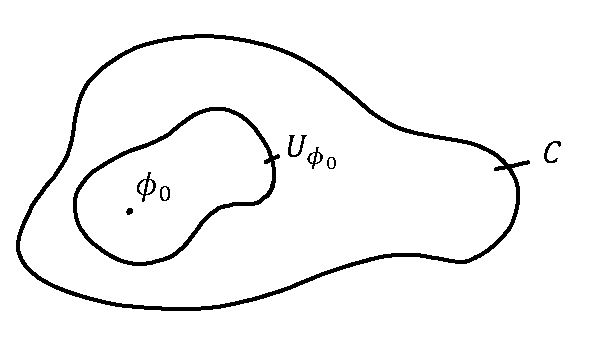
\includegraphics[width=0.5\textwidth]{Pictures/Linearization} 
   	  			\caption{Intrinsically, searching a variation of a solution $\gamma_0\in \Sol$ which solve the disturbed motion equation is equivalent to find the intersection of the perturbed solution with a local neighbourhood of $\Gamma_0$ : $U_{\gamma_0}\cap\ker(P_\epsilon)$ .}
		\end{figure}		
		
		The crucial point of the Peierls' procedure  is to select among all the possible solution of the perturbed motion $P_\epsilon$ that configuration which can be constructed by a variation of some fixed solution of the non-perturbed dynamics $\gamma_0 \in \Sol$.
		In this sense the problem results a \emph{"linearization"} inasmuch the  search of such solution is restricted to a local neighbourhood of the "point" $\gamma_0\in \Sol$.

		Previously the choice to consider only the linear variation was quite natural but in the general case this preferential restriction is no longer possible.
		A way to  recover a notation similar to \ref{PerturbedSolution} is to work patchwise choosing a coordinate representation.
		Fixed a solution $\gamma_0 \in \Sol$ and a local trivializing chart $(A, \phi_A)$ such that $A\cap \ran(\gamma_0) \neq \emptyset$ we can define a local infinitesimal variation by acting on his components:
		\begin{displaymath}
			\gamma_\lambda ^{\, i}(x) = \gamma_0^{\, i}(x) + \lambda \eta^i(x) \qquad \forall x\in \pi(A)
		\end{displaymath}
		where $ \gamma_0^{\, i}$ are the component of the unperturbed solution in the open set $A$ and $\eta^i\in \real^q$ is a generic real q-ple ( q is the dimension of the typical fiber manifold).
		$\lambda$ is a real parameter that has to be "sufficiently small" in order to guarantee that the range of $\gamma_\lambda$ is properly contained in $A$.
		In other words the construction of the linear variation, that for linear field theories could be done in a global way, in the general case can be recovered only locally variating the components.
		
		Therefore is possible to define the effect of the a disturbance locally, searching local section $\gamma_\epsilon^{\, i} = \gamma_0^{\, i} + \epsilon \eta^{i}$ solving the disturbed dynamic equation up to the first order in $\epsilon$ i.e. 
		\begin{displaymath}
			\big[ P_\epsilon \big] \gamma_\epsilon^{\,i} = o(\epsilon)
		\end{displaymath}
		where $\big[ P_\epsilon \big] $ has to be intended as the coordinate representation of the operator with restricted domain to the local sections $\Gamma^\infty(A)$.
		\begin{observation}
		W.l.o.g has been taken the the same scalar $\epsilon$  to modulate both the perturbation $\gamma_\epsilon$ that the disturbance on the motion operator.
		On the contrary consider two different parameter is immaterial since only the smaller should be taken in account.
		\end{observation}

		From the explicit equation of the perturbed solution: 
		\begin{displaymath}
			\biggr(\big[P\big] + \epsilon\big[Q_\chi\big] \biggr) \big(\gamma_0^{\,i}+\epsilon \eta^i \big) = o(\epsilon)
		\end{displaymath}
		follows an equation on the components of the local perturbation.
		In  this case has to be dealt with the problem of non-linearity not only for Euler-Lagrange operator $Q_\chi$ but also for $P$.
		Arresting the expension to the first order in $\epsilon$ results:
		\begin{equation}\label{PeierlJacobiEqNonLin}
			\biggr[P_{\gamma_0}^{\, lin} \biggr] \eta^i(x) = -\biggr(Q_\chi(\gamma_0)\biggr)(x)
		\end{equation}
		the \emph{Jacobi equation} on the unperturbed solution $\gamma_0\in \Sol$.
		\begin{observation}
			We've moved from an operator $P$  definited on  $\Conf$ to an operator  $P_{\gamma_0}^{\, lin}  $ defined on the space of variation.
			From a global point of view this variation can be seen as the tangent vector i.e. s  $\eta \in T_{\gamma_0}\Conf$.
			In the case of the linear system this passage was unnecessary, the Jacobi equation was directly defined on $\Conf$ since, for linear system, any section could be seen as a generator of an infinitesimal variation.
			This behaviour mimics perfectly what happens in ordinary classical mechanics where the configuration space of a linear system is a vector space i.e a "flat" manifold\footnote{In sense that admits a global coordinate chart.} which is isomorphic to his tangent space in every point.
		\end{observation}
		
		Provided that the linearized motion operator (which is now properly a linear partial differential operator) is Green-Hyperbolic, the Peierels construction can continue as before.
		Has to be noted that now the advanced/retarded perturbation are formally identical to the former:
		\begin{displaymath}
			\eta^{\pm\, i} = G^\pm \big( - Q_\chi \gamma_0^{\, j})
		\end{displaymath}
		with the important difference that $G^\pm$ are now the Green operators of the linearized motion operator and depend on the fixed solution $\gamma_0^{\, j}$.
		
		In conclusion the perturbed solution:
		\begin{displaymath}
			\gamma_{\chi}^{\pm\,i} = \gamma_0^{\, i} \pm G^\pm \big( -Q_\chi \gamma_0^{\,j}\big)
		\end{displaymath}
		has to be intended as the "glueing" of all the local chart representations covering the chosen solution.

	\subsubsection{Example: Finite Dimensional Case} 
		As an example of such process we can consider a \emph{field of curves} i.e. an ordinary classical mechanical system in the field theoretic picture.
		We have shown in section \ref{MechanicsAsAField} that such systems are generally non linear: the configuration bundle is not a vector one and then linearity of $P$ cannot be defined .
	 	\begin{figure}[h!]\label{GraphicAdvRetSol}
				  \centering
   			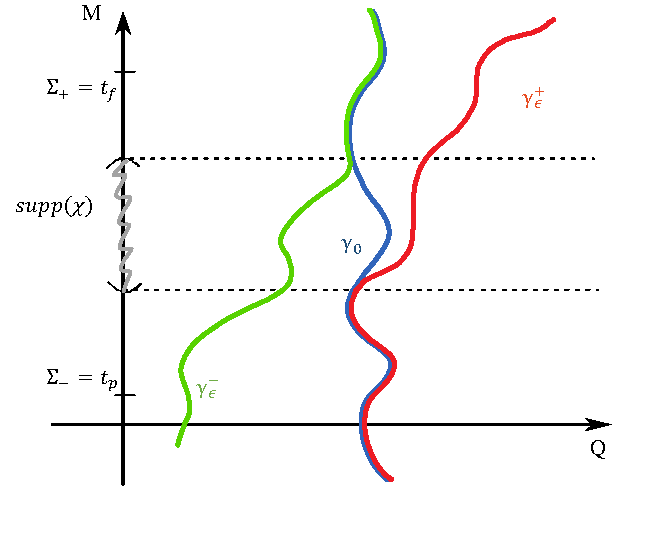
\includegraphics[width=0.5\textwidth]{./Pictures/AdvRetSol} 
   	  		\caption{Picture of the perturbed solution in case of a finite dimensional system.}
		\end{figure}			
		
		However the base manifold is very simple. Indeed $M= \Real$ can be seen as a trivial globally-hyperbolic space-time where every real scalar $t\in M$ is a Cauchy surface.
		This allows us to specify the above equations in a more intuitive way:
		\begin{itemize}
			\item $\gamma_0^{\, j}$ is a simple local chart representation of the curve.
			\item for a suitable small $\epsilon$  $\gamma_0^{\, j}$ and $\gamma_{\chi}^{\pm\,i} $ can be pictured in the same local chart.
			\item the variation $\eta^\pm$ is then the field over the unperturbed curve whose components compute the separation between $\gamma_0$ an $\gamma_{\chi}^{\pm} $
		\end{itemize}
	
	 	
\end{document}